\section{Reusability and Extensibility}
\label{sec:gaia_reuse}

%As mentioned earlier, reusing not only accelerates the design process for beginners but also eases the design of repeated parts within a single animation.
%The central concept behind \gaia's reusability lies in decoupling animation designs from specific animated targets, drawing inspiration from the bridge pattern in OOP.
%In this section, we will delve into target type abstraction and demonstrate how our target type system operates within the animation specification.

Some infographics have similar semantic components, and animations of these components are also similar.
Reusing these animation benefits creating progress \cite{thompson2020understanding}.
However, their structures in the form of SVG differ from each other.
For example, the order of elements or hierarchy made by \code{<g>} might vary inside SVG code. 
Reusing animation across different instances requires a unified target abstraction.
In the previous section, we introduce the attribute \code{target} in animation spec, discussing how \gaia{} manages the targeted elements of each \aniunit{}.
In fact, these target specs are performed on an abstraction layer, as we call \textit{virtual target model}, instead of original SVGs.
In this section, we will discuss the target abstraction and explain how it enables reusability and extensibility of \gaia{} animation spec.

\subsection{Target Abstraction and Reusing}
\label{sec:target_type}

% We follow the intuition that the animated targets have a tree-like hierarchy, which is similar to the SVG DOM tree or the concept of scene graph \cite{satyanarayan2015reactive}.
% So the target abstraction in \gaia{} is the same as the target model introduced in \autoref{ssec:gaia_ani_target}, which is a tree-like structure formed by groups.
% The difference is that for each group node in the target abstraction, we assign a type to it, which is called target type.
% Each type of animated target, defined by target type spec (introduced in \autoref{ssec:target_type_decl}), has a set of declared components, which represents the types of its children.
% Then a concrete \textit{target type tree} can be created (\autoref{fig:virtual_target_model}(A)), which further defines the backbone of the virtual target model.
% Original SVG elements are appended to corresponding nodes in the virtual target model.
% \autoref{fig:virtual_target_model}(B) shows an example for the animated infographic and its SVG in \autoref{fig:virtual_target_model}(C).
% One of the advantages of this design is that users can still use id/class on the original elements to select animation targets~\footnote{Design of the virtual target model can be in other forms and replaced in our implementation smoothly.}.
% From the point of view of the original SVG, the virtual target model is a kind of reformatting.
% This process is done by another JSON spec named binder (\autoref{ssec:binder_spec}). 

The virtual target model employs the same target selection mechanism in \autoref{ssec:gaia_ani_target}.
However, in the virtual target model, elements in the list of target selection are not the original SVG elements.
To provide sufficient abstraction capability, the design of the virtual target model should be carefully considered.
We found that the animated targets have a tree hierarchy, which is similar to the SVG DOM tree or the concept of scene graph \cite{satyanarayan2015reactive}.
According to the insights from Kim \etal~\cite{kim2020gemini}, users might specific sub-elements like \textit{the x-axis title}.
Motivated by these findings, we design the target abstraction as a tree-like structure to support such expressions. 
Specifically, the target abstraction is a tree shown on the left side of \autoref{fig:virtual_target_model}, as we call \textit{target type tree}.

\begin{figure}[h]
  \centering
  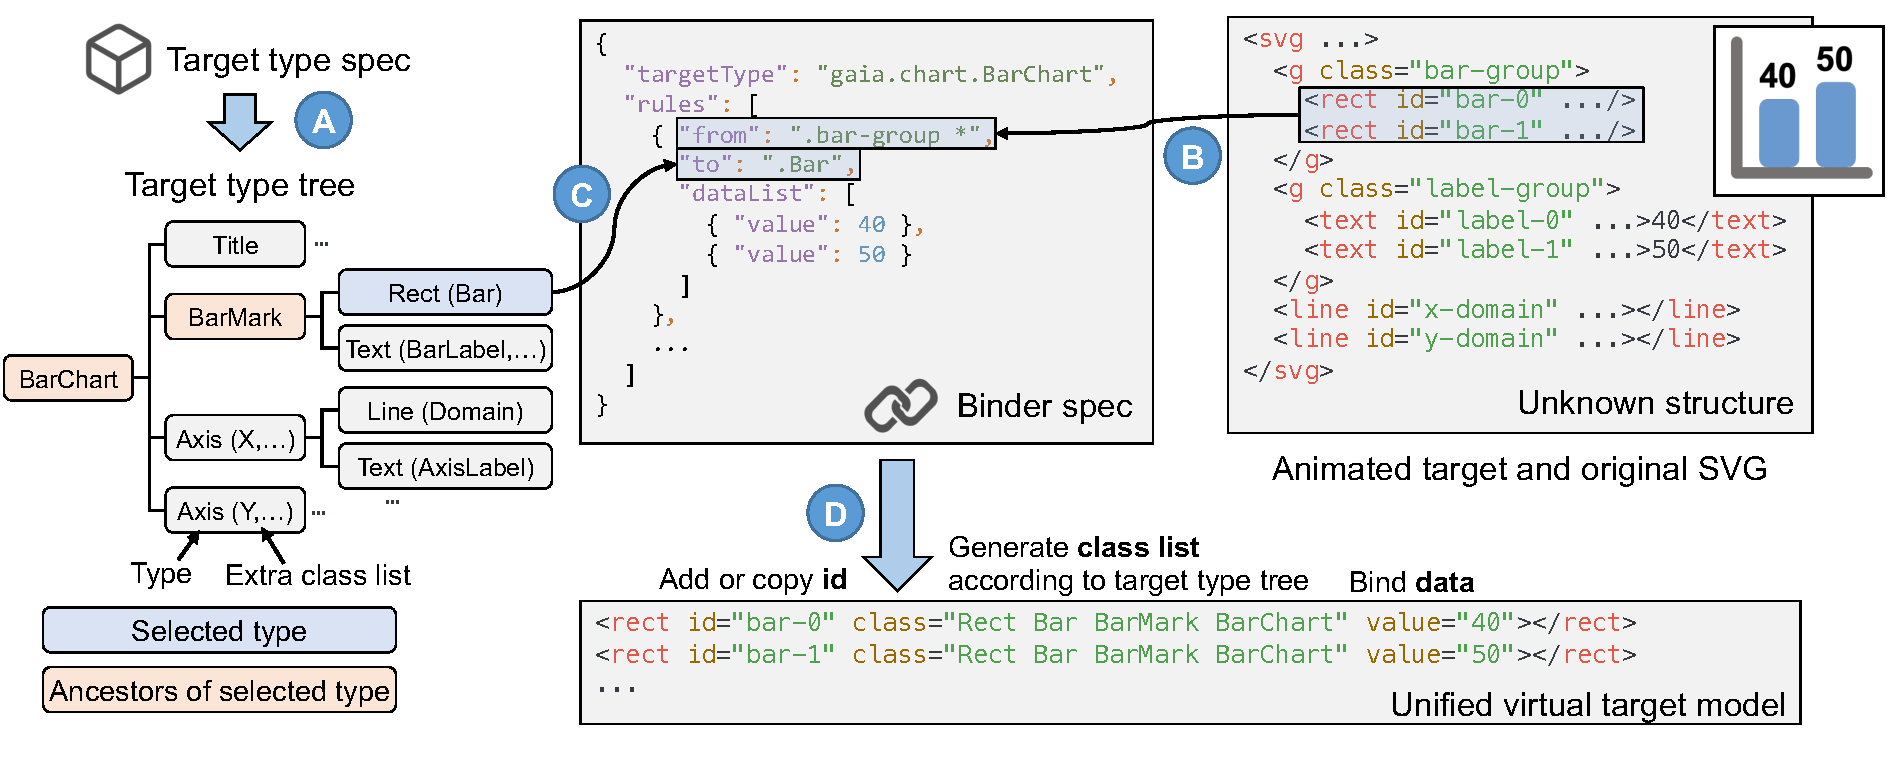
\includegraphics[width=\linewidth]{figs/target_workflow.pdf}
  \caption{Steps to create a virtual target model, which can be used as a unified representation of a class of infographics.}
%  \Description{Steps to create a virtual target model, which can be used as a unified representation of a class of infographics.}
  \label{fig:virtual_target_model}
\end{figure}

Target type trees are defined using a JSON-style spec, named target type spec (\autoref{fig:virtual_target_model}(A), introduced in \autoref{ssec:target_type_decl}).
Then, with a binder spec (\autoref{ssec:binder_spec}), the original SVG elements can be bound to a semantic type by linking it to a node of the target type tree (\autoref{fig:virtual_target_model}(B, C)).
Then a virtual target model can be generated (\autoref{fig:virtual_target_model}(D)), which is a list of virtual SVG elements.

With the virtual target model, all animated instances, \ie SVG, of the same type can be represented as a list of elements with class lists defined by the target type tree.
The target attributes in animation spec are applied on this virtual layer, which enables the reusability of animation spec regardless of the structure of SVGs.
The expert designers can represent and share their animation designs as \aniclass{}es and end users can simply reuse them using \code{ref} keyword.

\subsection{Target Type Spec}
\label{ssec:target_type_decl}

The target type spec, which defines the target types and their components, is also in JSON style.
Inspired by the object declaration in JSON schema \cite{json-schema-org}, the target type spec can declare other target types as its components via \code{ref} attribute.
As shown in \autoref{fig:type_spec}(A-C), the type declaration of BarChart contains components defined in other target type spec, declared a target type tree for BarChart shown in \autoref{fig:virtual_target_model}(A).
All these specs can be reused to form other target types, such as LineChart or Timeline.
\gaia{} manages these target types via packages and provides a set of target types for common infographics and their components.

\begin{figure}[h]
  \centering
  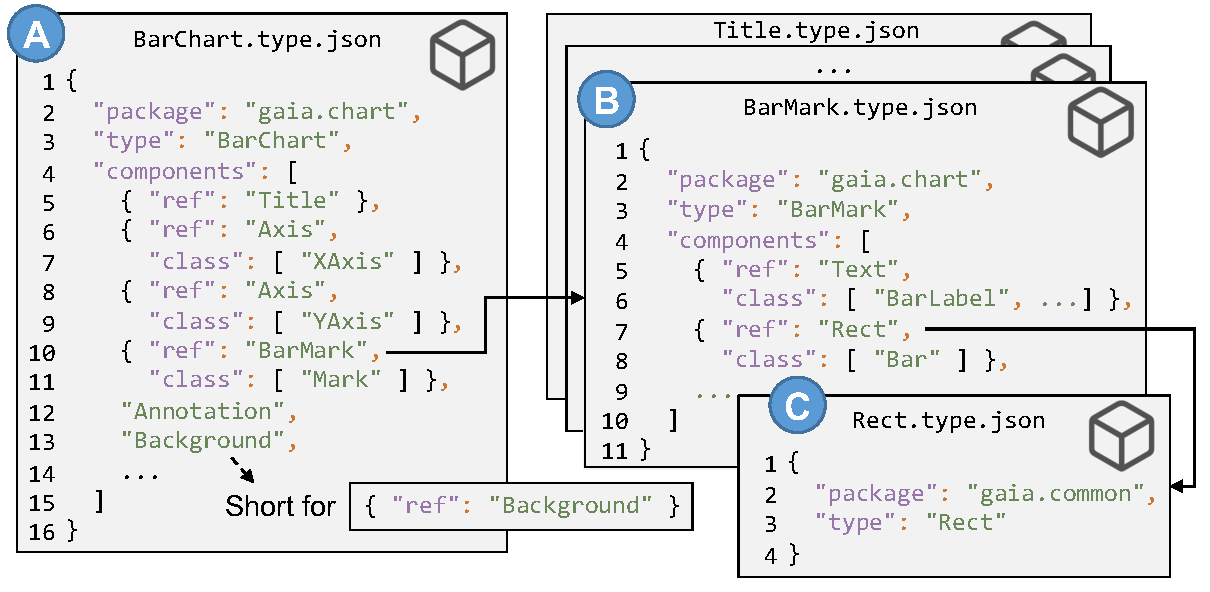
\includegraphics[width=\linewidth]{figs/target_type_spec.pdf}
  \caption{Target type can be declared using target type specs (A-C) with a specified type name and components. (D) lists the attributes used in target type spec.}
%  \Description{Target type can be declared using target type specs (A-C) with a specified type name and components. (D) lists the attributes used in target type spec.}
  \label{fig:type_spec}
\end{figure}

\autoref{fig:type_spec}(D) gives a detailed explanation of attributes in target type spec.
Notice that \code{package} can be used to avoid name conflicts.
In this case, these specs are in the same package so no import is needed (common types don't need to import).
The name of the type and class list declared in components will be used in the class list of nodes in the target type tree.


\subsection{Binder Spec}
\label{ssec:binder_spec}

Binder spec is used to bind the original SVG elements to the target type tree, and then generate the virtual target model.
As shown in \autoref{fig:virtual_target_model}, a binder spec contains attributes \code{targetType} and \code{rules}.
The value of \code{targetType} determines the target type tree to use.
Each rule in the \code{rules} (1) selects a set of elements in the original SVG by a CSS selector in \code{from}, (2) selects exactly one node in the target type tree by a CSS selector in \code{to}, and (3) binds the data to each element one by one according to the \code{dataList} attribute.
Element id can also be set if needed. 
The result is called virtual target model, which is a list of transformed SVG elements.
Each element has (1) id (\gaia{} will generate one automatically if no id is available), (2) a list of class names that come from the selected type node and its ancestors, and (3) data written to the attributes of the element.
This list will be the root selection of the animation spec, and the \code{target} of the \aniunit{} at \code{main} will be applied to it.


\subsection{Using Animation Spec as Template}
\label{ssec:extend_template}

One \aniclass{}, introduced in \autoref{ssec:aniclass_aniunit}, can be directly stored as a template and reused in other animation specs or further be a part of another template.
Notice that \aniclass{} can be declared without any concrete instance because the target is declared according to the virtual target model.
Now taking the animation in \autoref{fig:ani_hierarchy} as an example, we discuss how \aniclass{}es in \gaia{} cooperate to represent a complex animation.
Notice that end users, only need to specify the top \aniclass{} for customizability, where they can freely reuse animations from expert designers, so the progress is accelerated greatly.

\begin{figure}[h]
  \centering
  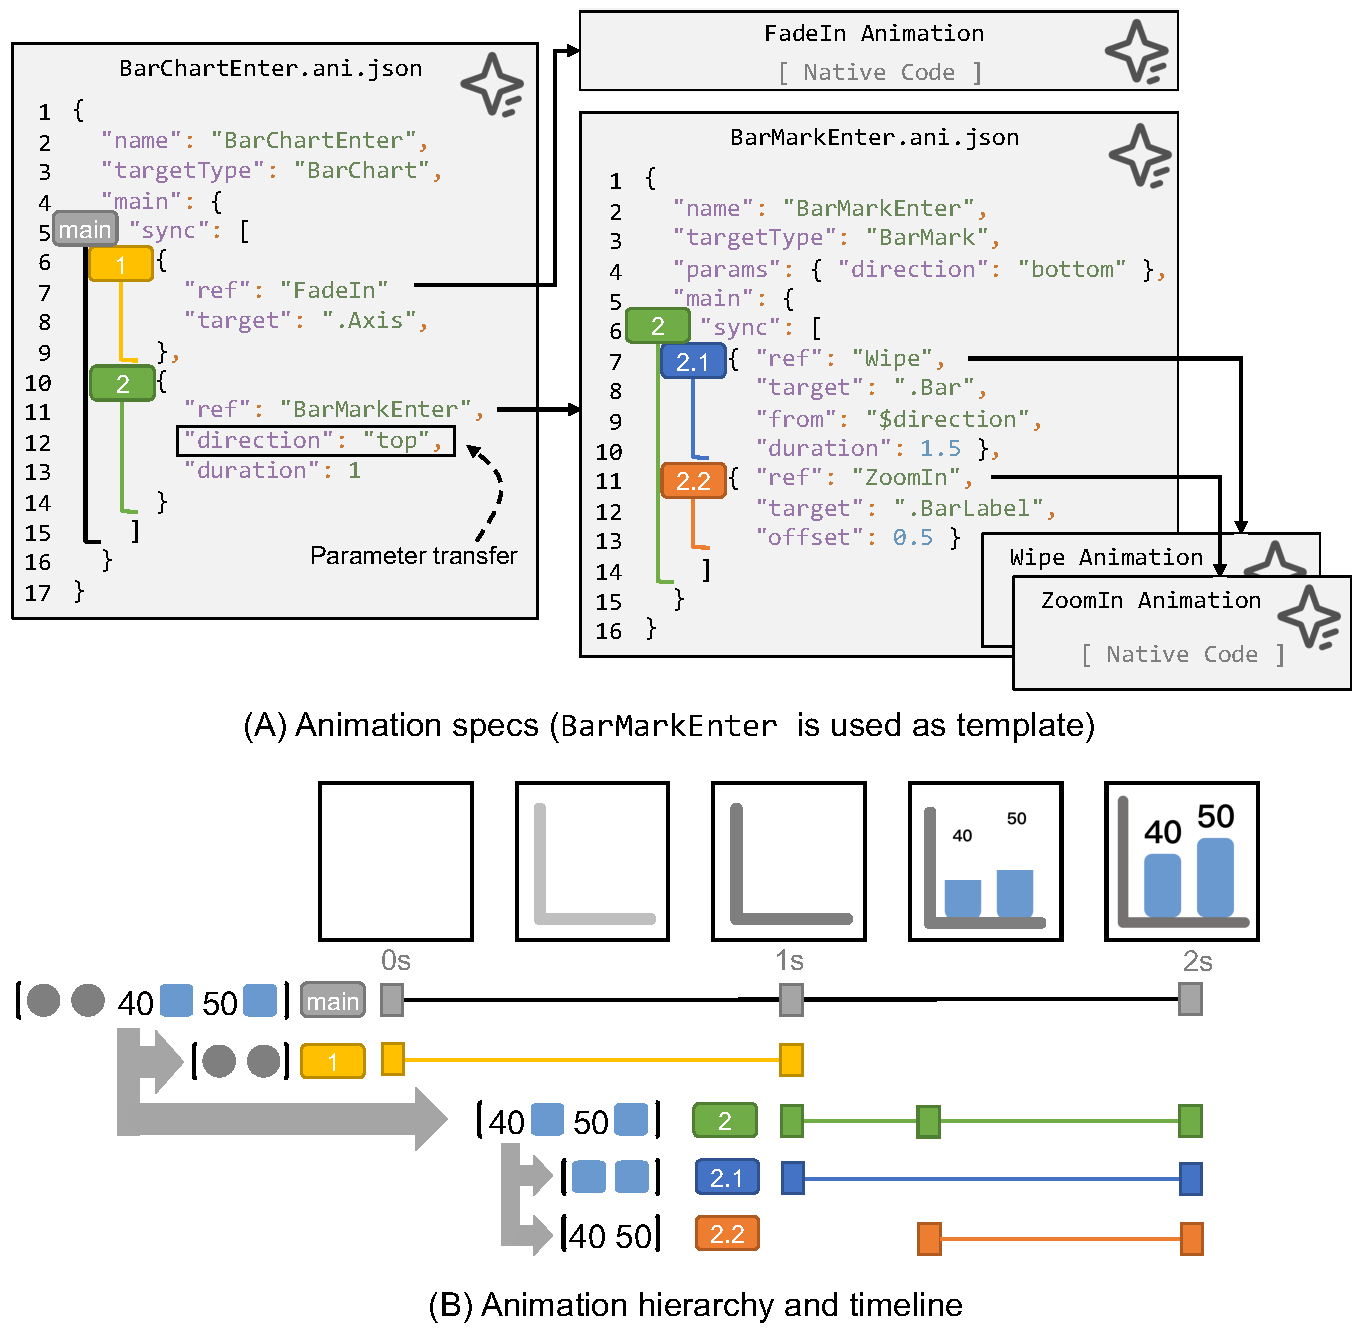
\includegraphics[width=\linewidth]{figs/ani_hierarchy.pdf}
  \caption{An example of using animation spec as a template to declare and instantiate a complex animation.}
%  \Description{An example of using animation spec as a template to declare and instantiate a complex animation.}
  \label{fig:ani_hierarchy}
\end{figure}

\autoref{fig:ani_hierarchy}(A) shows an \aniclass{} designed for BarChart. 
It refers to two sub-\aniclass{}es, FadeIn on axis components and BarMarkEnter (as same as the spec in \autoref{fig:ani_spec}(A)).
The BarMarkEnter further refers to other \aniclass{}es stored in the library, though form an animation hierarchy.
In this case, the animation spec BarMarkEnter declared using JSON is composited as a sub-animation.
It picks targets from the outer scope and the timing settings are dominated as well (rescaling duration if needed).
Parameters set in the outer scope will be transferred to the sub-animation.
Applying an SVG example, the final timeline and selected elements for each declared \aniunit{}s are shown in \autoref{fig:ani_hierarchy}(B).

Attributes of \textit{Class} specify more information of one \aniclass{}. 
Attribute \code{import} specifies other \aniclass{}s used by \code{ref} keyword, which prevents name conflicts (common \aniunit{}s don't need to import). 
\aniclass{} \code{name} is used when other \aniclass{}s refer to and reuse it (\code{"Main"} as default).
The target type that this \aniclass{} associates with is declared by \code{targetType}.
Attribute \code{params} allow users to set the parameters passed in when reusing, leaving the customizability of \aniclass{}s.
An example is shown in line 12 in \autoref{fig:ani_hierarchy}(A).

We want to emphasize that this mechanism does not rely on any concrete infographic instance. 
For example, in this case, users create an \aniclass{} for BarChart via combining existing designs for components, \ie axes and marks, without referring to a given bar chart SVG.
Then this \aniclass{} can also be registered to the library and used later.
All these things can be done in, but not limited to, a JSON-style spec, to implement the extensibility of \gaia{}.
Designers can share their animation designs with other users for reusing without the involvement of \gaia{}'s developers.

